\chapter{Chi-square Distribution ($X \sim \chi^2_k$) \cite{ism-1,wiki/Chi-squared_distribution}} \label{Chi-square Distribution}

\begin{table}[H]
    \begin{minipage}{0.49\linewidth}
        \begin{figure}[H]
            \centering
            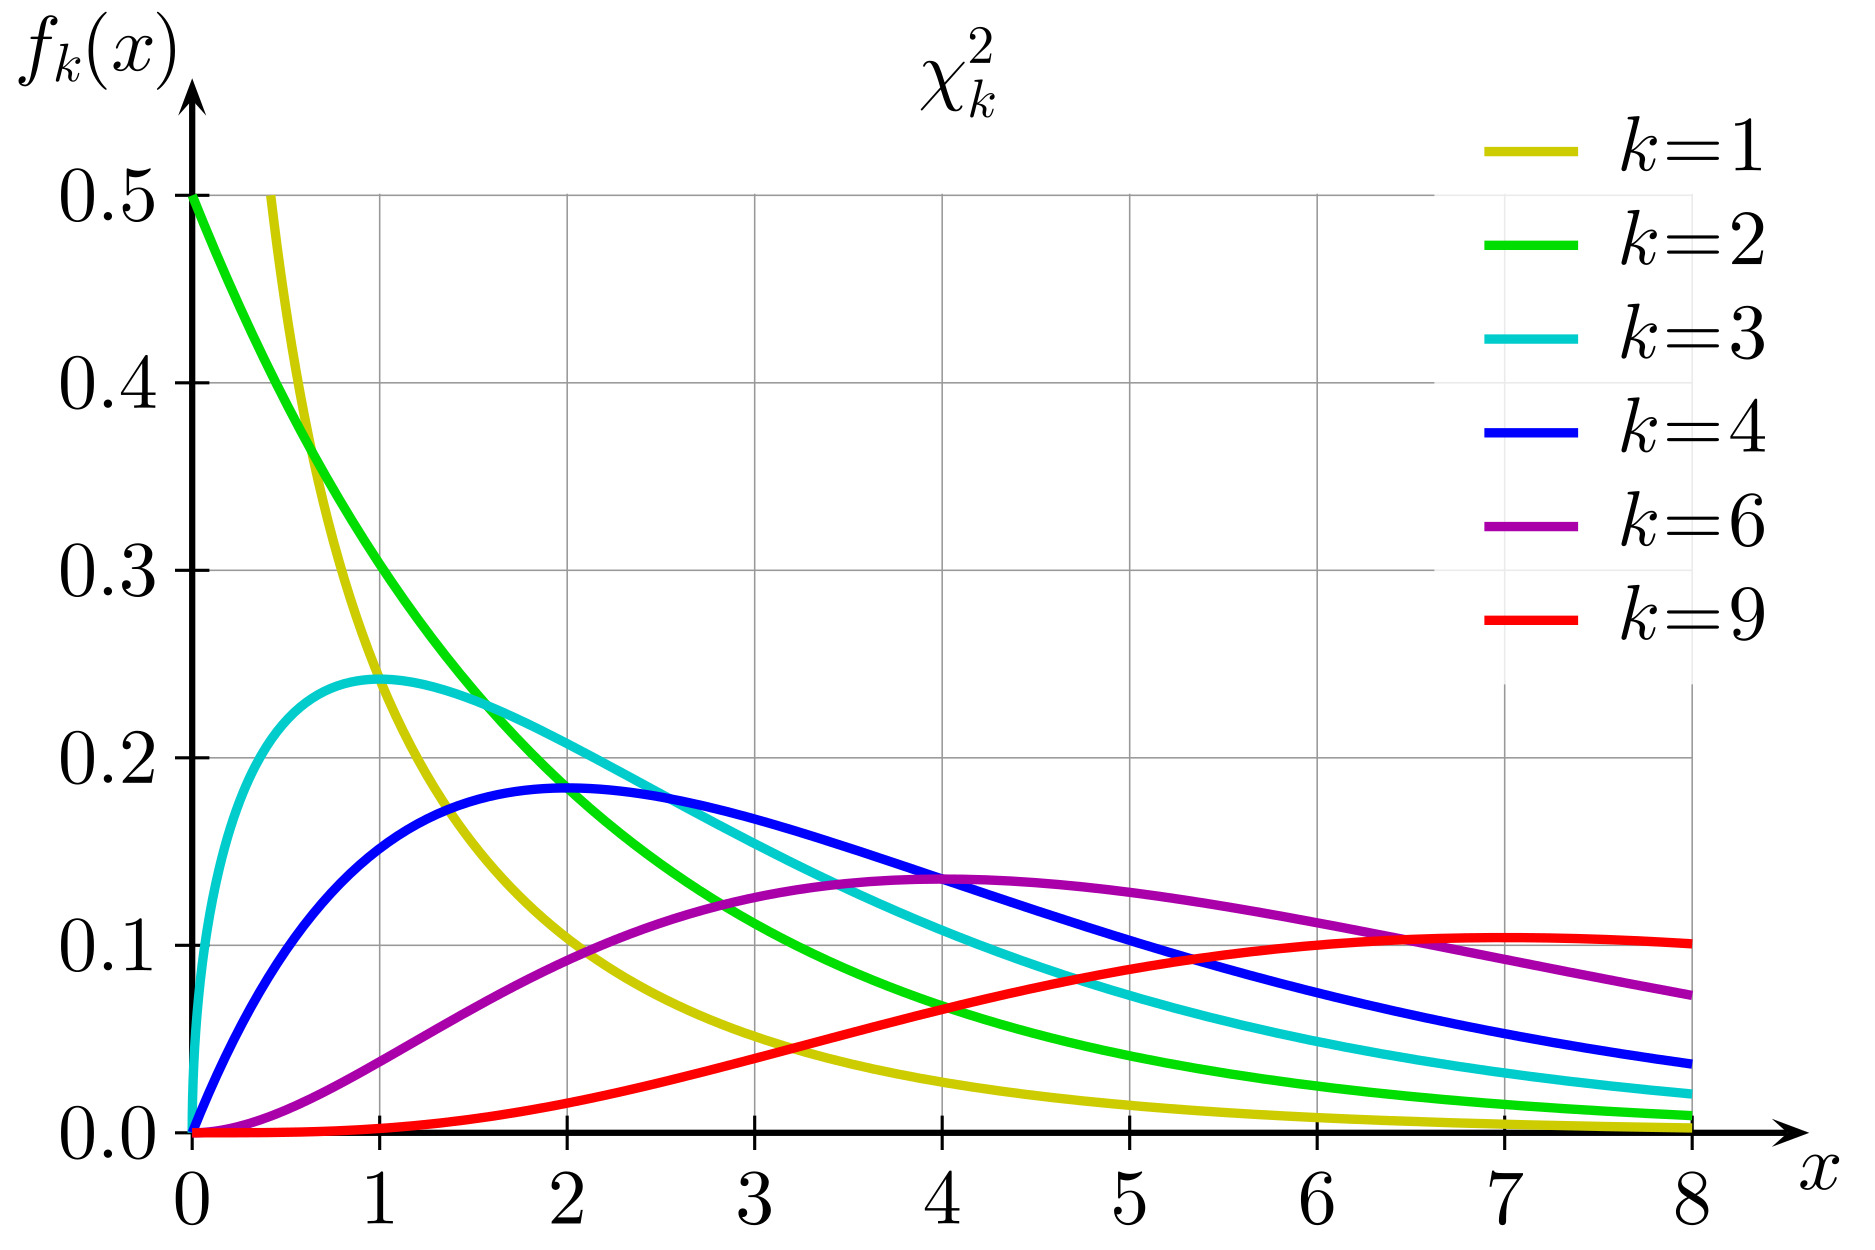
\includegraphics[width=\linewidth, height=4cm, keepaspectratio]{Pictures/distributions/Chi-square_pdf.jpg}
            \caption{Chi-square Distribution: PDF}
        \end{figure}
    \end{minipage}
    \hfill
    \begin{minipage}{0.49\linewidth}
        \begin{figure}[H]
            \centering
            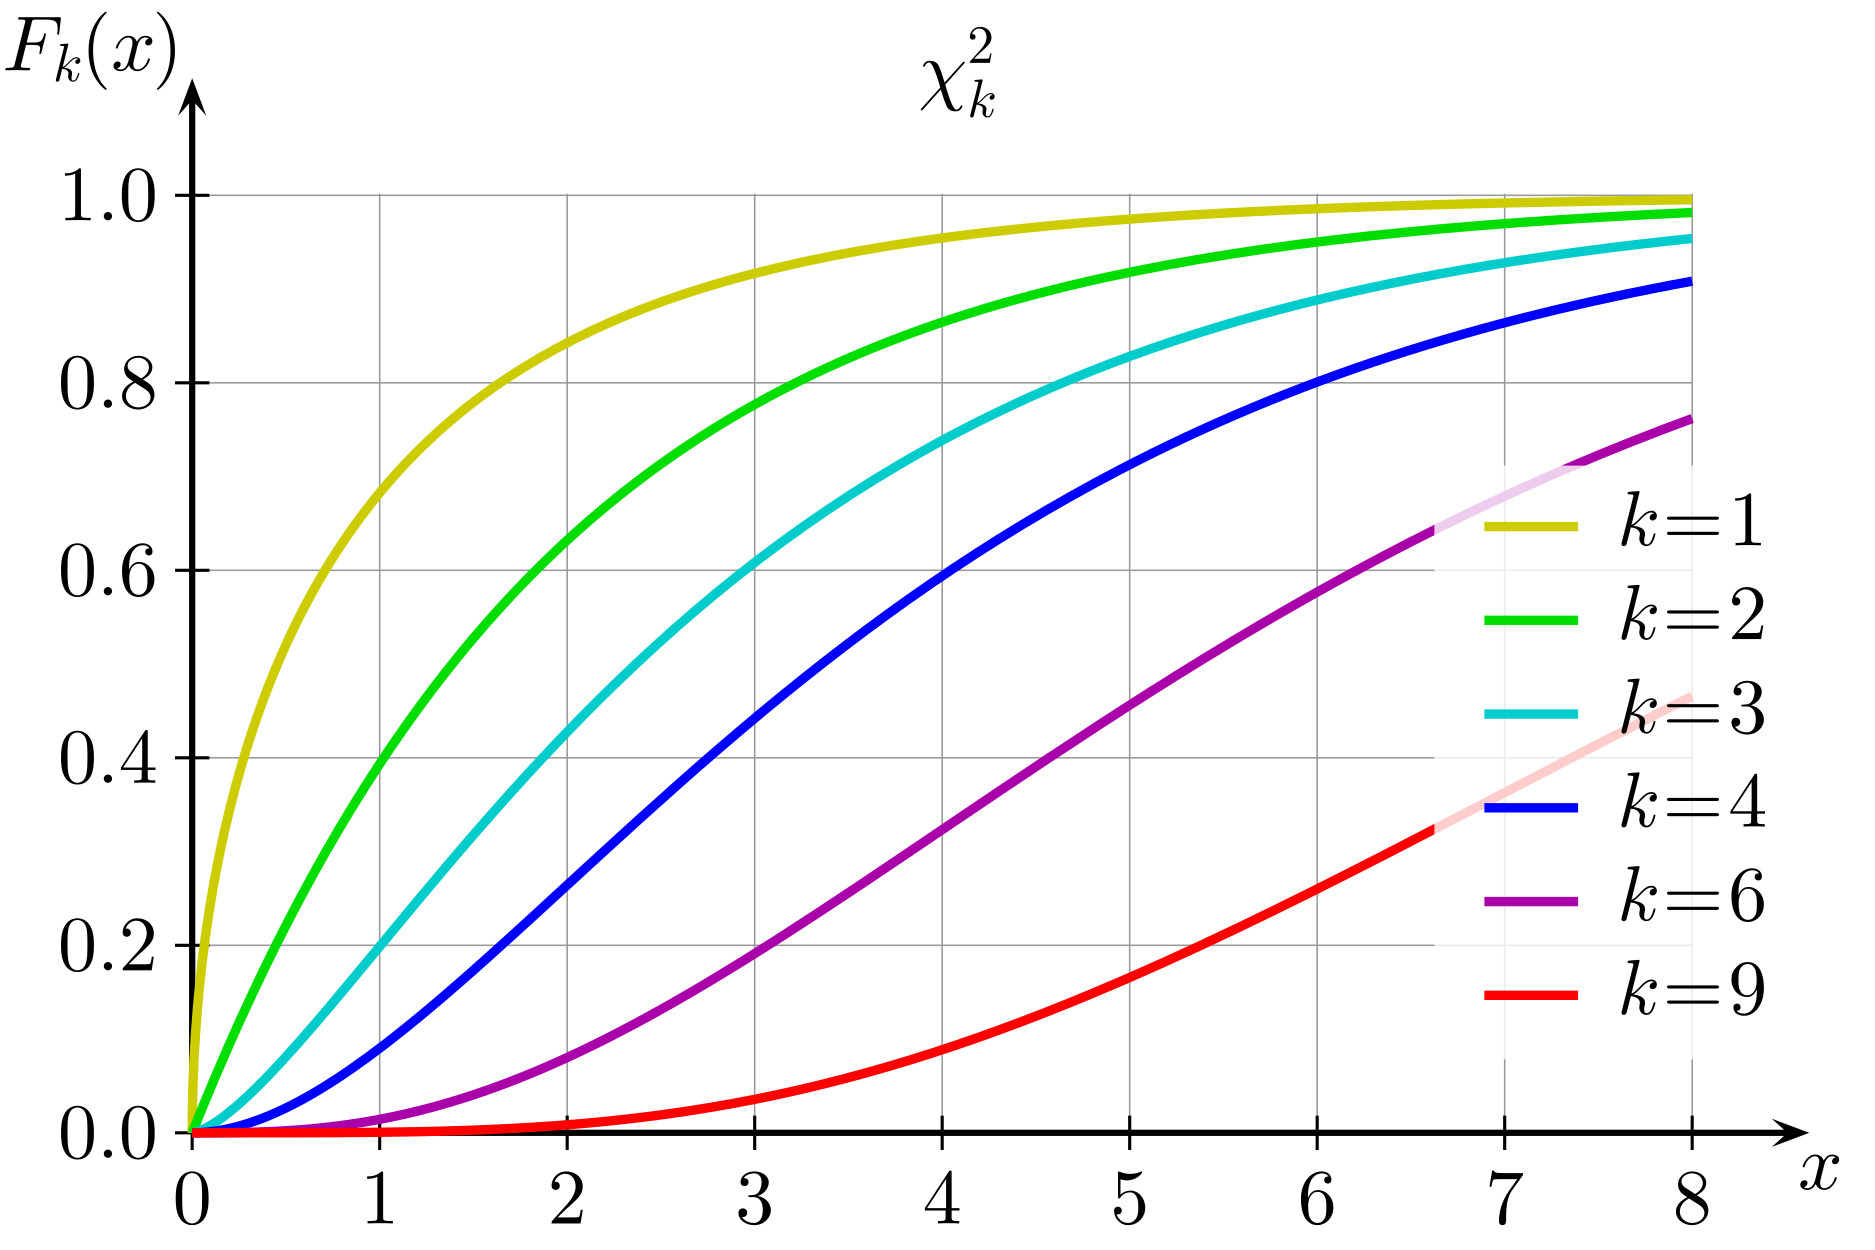
\includegraphics[width=\linewidth, height=4cm, keepaspectratio]{Pictures/distributions/Chi-square_cdf.jpg}
            \caption{Chi-square Distribution: CDF}
        \end{figure}
    \end{minipage}
\end{table}

\begin{customTableWrapper}{2}
\begin{longtable}{|m{6cm}|p{9cm}|}
    \hline
    \customTableHeaderColor
    \multicolumn{2}{|c|}{\textbf{Chi-square Distribution - Info} \cite{wiki/Chi-squared_distribution}} \\
    \hline\endfirsthead

    \hline
    \customTableHeaderColor
    \multicolumn{2}{|c|}{\textbf{Chi-square Distribution - Info - contd.} \cite{wiki/Chi-squared_distribution}} \\
    \hline\endhead
    
    \hline\endfoot
    \hline\endlastfoot

    \textbf{Notation} &
    ${ \chi ^{2}(k)\;}$ or ${ \chi _{k}^{2}\!}$
    \\ \hline

    \textbf{Statistical parameters} & 
    ${ k\in \mathbb {N} ^{*}~~}$ (known as "degrees of freedom")
    \\ \hline
    
    \textbf{Support} &
    ${ x\in [0,+\infty )\;}$
    \\ \hline

    \textbf{Probability Density Function (PDF)} & 
    ${ {\dfrac {1}{2^{k/2}\Gamma (k/2)}}\;x^{k/2-1}e^{-x/2}\;}$
    \\[1ex] \hline
    
    \textbf{Cumulative distribution function (CDF)} & 
    ${ {\dfrac {1}{\Gamma (k/2)}}\;\gamma \left({\dfrac {k}{2}},\,{\dfrac {x}{2}}\right)\;}$
    \\ \hline

    \textbf{Mean} & 
    $k$
    \\[1ex] \hline

    \textbf{Median} & 
    ${ \approx k{\bigg (}1-{\dfrac {2}{9k}}{\bigg )}^{3}\;}$
    \\[1ex] \hline

    \textbf{Mode} & 
    ${ \max(k-2,0)\;}$
    \\ \hline

    \textbf{Variance} &
    $2k$
    \\[1ex] \hline

    \textbf{Skewness} &
    ${ {\sqrt {\dfrac{8}{k}}}\,}$
    \\[1ex] \hline

    \textbf{Excess kurtosis} &
    ${ {\dfrac {12}{k}}}$
    \\[1ex] \hline

    \textbf{Entropy} &
    ${ {{\dfrac {k}{2}} +\log \left(2\Gamma {\Bigl (}{\dfrac {k}{2}}{\Bigr )}\right)+\left(1-{\dfrac {k}{2}}\right)\psi \left({\dfrac {k}{2}}\right)}}$
    \\[1ex] \hline

    \textbf{Moment-generating function (MGF)} &
    ${ (1-2t)^{-k/2}{\text{ for }}t<{\dfrac {1}{2}}\;}$
    \\[1ex] \hline

    \textbf{Characteristic function (CF)} &
    ${ (1-2it)^{-k/2}}$
    \\[1ex] \hline

    \textbf{Probability-generating function (PGF)} &
    ${ (1-2\ln t)^{-k/2}{\text{ for }}0<t<{\sqrt {e}}\;}$
    \\[1ex] \hline

\end{longtable}
\end{customTableWrapper}

\begin{enumerate}[itemsep=0.2cm]
    \item Confidence Interval:
    \begin{enumerate}[itemsep=0.2cm]
        \item $V_{n-1}^2 = (n-1)S^2/\sigma^2 \sim \chi_{n-1}^2$

        \item $p$th quantile of the chi-square distribution with $n - 1$ DOF: $x_p(f_{\chi^2})$

        \item $
            \hfill
            Pr(V_{n-1}^2 \leq x_p(f_{\chi^2})) = p
            \hfill
            Pr(V_{n-1}^2 > x_{1-p}(f_{\chi^2})) = p
            \hfill
        $

        \item $
            Pr(\sigma^2 < (n-1)S^2/x_{1-p}(f_{\chi^2})) = p 
        $

        \item $1 - 2p$ confidence interval for the variance $\sigma^2$ is:
        \[[
            (n-1)S^2/x_{1-p}(f_{\chi^2}), 
            \hspace{0.2cm}
            (n-1)S^2/x_{p}(f_{\chi^2})
        )\]

    \end{enumerate}

\end{enumerate}



\section{Inverse-Chi-square Distribution/ Inverted-chi-square distribution ($X \sim \chi^{-2}$) \cite{wiki/Inverse-chi-squared_distribution}} \label{Inverse-Chi-square Distribution/ Inverted-chi-square distribution}



\begin{table}[H]
    \begin{minipage}{0.49\linewidth}
        \begin{figure}[H]
            \centering
            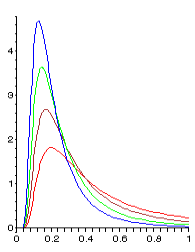
\includegraphics[width=\linewidth, height=4cm, keepaspectratio]{Pictures/distributions/Inverse_chi_squared_pdf.png}
            \caption{Inverse-Chi-square Distribution: PDF}
        \end{figure}
    \end{minipage}
    \hfill
    \begin{minipage}{0.49\linewidth}
        \begin{figure}[H]
            \centering
            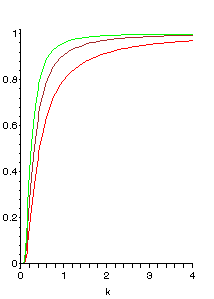
\includegraphics[width=\linewidth, height=4cm, keepaspectratio]{Pictures/distributions/Inverse_chi_squared_cdf.png}
            \caption{Inverse-Chi-square Distribution: CDF}
        \end{figure}
    \end{minipage}
\end{table}

\begin{customTableWrapper}{2}
\begin{longtable}{|m{6cm}|p{9cm}|}
    \hline
    \customTableHeaderColor
    \multicolumn{2}{|c|}{\textbf{Inverse-Chi-square Distribution - Info} \cite{wiki/Inverse-chi-squared_distribution}} \\
    \hline\endfirsthead

    \hline
    \customTableHeaderColor
    \multicolumn{2}{|c|}{\textbf{Inverse-Chi-square Distribution - Info - contd.} \cite{wiki/Inverse-chi-squared_distribution}} \\
    \hline\endhead
    
    \hline\endfoot
    \hline\endlastfoot

    \textbf{Statistical parameters} & 
    ${ \nu >0\!}$
    \\ \hline
    
    \textbf{Support} &
    ${ x\in (0,\infty )\!}$
    \\ \hline

    \textbf{Probability Density Function (PDF)} & 
    ${ {\dfrac {2^{-\nu /2}}{\Gamma (\nu /2)}}\,x^{-\nu /2-1}e^{-1/(2x)}\!}$
    \\[1ex] \hline
    
    \textbf{Cumulative distribution function (CDF)} & 
    ${ \Gamma \!\left({\dfrac {\nu }{2}},{\dfrac {1}{2x}}\right){\bigg /}\,\Gamma \!\left({\dfrac {\nu }{2}}\right)\!}$
    \\ \hline

    \textbf{Mean} & 
    ${ {\dfrac {1}{\nu -2}}\!}$ for ${ \nu >2\!}$
    \\[1ex] \hline

    \textbf{Median} & 
    ${ \approx {\dfrac {1}{\nu {\bigg (}1-{\dfrac {2}{9\nu }}{\bigg )}^{3}}}}$
    \\[1ex] \hline

    \textbf{Mode} & 
    ${ {\dfrac {1}{\nu +2}}\!}$
    \\ \hline

    \textbf{Variance} &
    ${ {\dfrac {2}{(\nu -2)^{2}(\nu -4)}}\!}$ for ${ \nu >4\!}$
    \\[1ex] \hline

    \textbf{Skewness} &
    ${ {\dfrac {4}{\nu -6}}{\sqrt {2(\nu -4)}}\!}$ for ${ \nu >6\!}$
    \\[1ex] \hline

    \textbf{Excess kurtosis} &
    ${ {\dfrac {12(5\nu -22)}{(\nu -6)(\nu -8)}}\!}$ for ${ \nu >8\!}$
    \\[1ex] \hline

    \textbf{Entropy} &
    ${ {\dfrac {\nu }{2}}\!+\!\ln \!\left({\dfrac {\nu }{2}}\Gamma \!\left({\dfrac {\nu }{2}}\right)\right)} { \!-\!\left(1\!+\!{\dfrac {\nu }{2}}\right)\psi \!\left({\dfrac {\nu }{2}}\right)}$
    \\[1ex] \hline

    \textbf{Moment-generating function (MGF)} &
    ${ {\dfrac {2}{\Gamma ({\dfrac {\nu }{2}})}}\left({\dfrac {-t}{2i}}\right)^{\!\!{\dfrac {\nu }{4}}}K_{\dfrac {\nu }{2}}\!\left({\sqrt {-2t}}\right)}$ does not exist as real valued function
    \\[1ex] \hline

    \textbf{Characteristic function (CF)} &
    ${ {\dfrac {2}{\Gamma ({\dfrac {\nu }{2}})}}\left({\dfrac {-it}{2}}\right)^{\!\!{\dfrac {\nu }{4}}}K_{\dfrac {\nu }{2}}\!\left({\sqrt {-2it}}\right)}$
    \\[1ex] \hline

\end{longtable}
\end{customTableWrapper}


\begin{enumerate}
    \item The inverse-chi-squared distribution (or inverted-chi-square distribution) is the probability distribution of a random variable whose multiplicative inverse (reciprocal) has a chi-squared distribution

\end{enumerate}


\section{Scaled inverse chi-squared distribution $X \sim \chi^{-2}(\nu, \tau^2)$ \cite{wiki/Scaled_inverse_chi-squared_distribution}} \label{Scaled inverse chi-squared distribution}

\begin{table}[H]
    \begin{minipage}{0.49\linewidth}
        \begin{figure}[H]
            \centering
            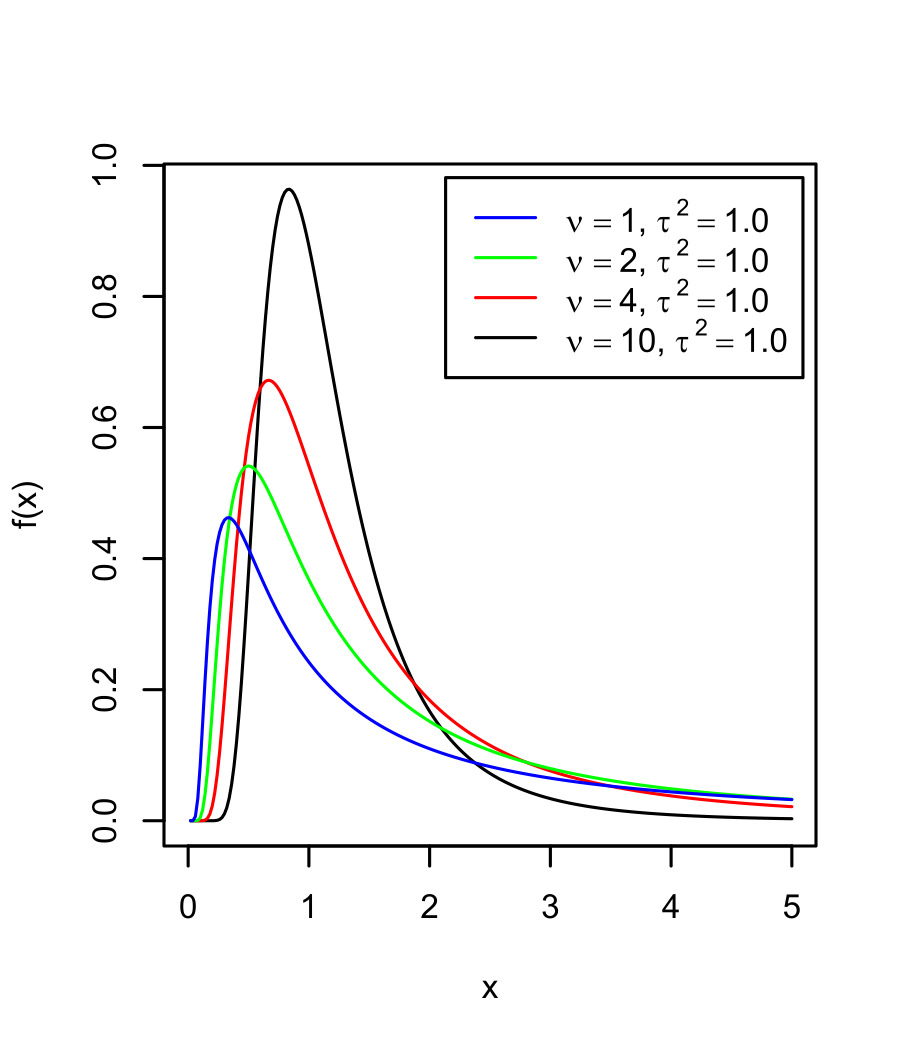
\includegraphics[width=\linewidth, height=4cm, keepaspectratio]{Pictures/distributions/Scaled_inverse_chi_squared_pdf.jpg}
            \caption{Scaled inverse chi-squared distribution: PDF}
        \end{figure}
    \end{minipage}
    \hfill
    \begin{minipage}{0.49\linewidth}
        \begin{figure}[H]
            \centering
            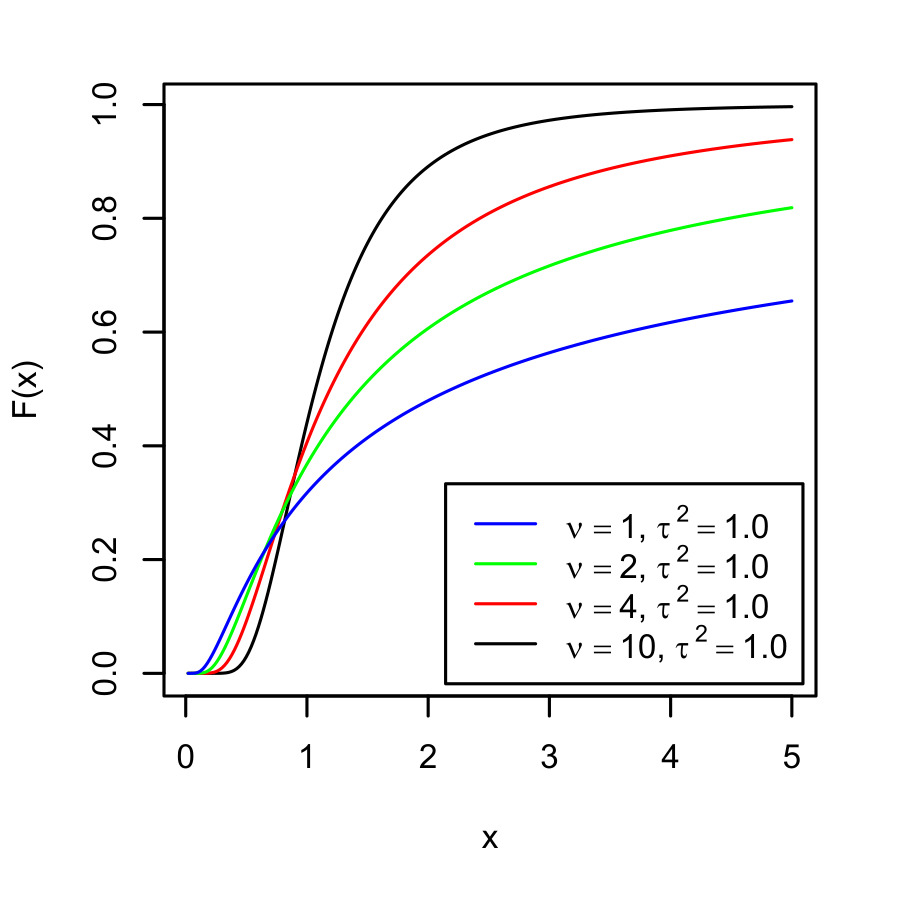
\includegraphics[width=\linewidth, height=4cm, keepaspectratio]{Pictures/distributions/Scaled_inverse_chi_squared_cdf.jpg}
            \caption{Scaled inverse chi-squared distribution: CDF}
        \end{figure}
    \end{minipage}
\end{table}

\begin{customTableWrapper}{2}
\begin{longtable}{|m{6cm}|p{9cm}|}
    \hline
    \customTableHeaderColor
    \multicolumn{2}{|c|}{\textbf{Scaled inverse chi-squared distribution - Info} \cite{wiki/Scaled_inverse_chi-squared_distribution}} \\
    \hline\endfirsthead

    \hline
    \customTableHeaderColor
    \multicolumn{2}{|c|}{\textbf{Scaled inverse chi-squared distribution - Info - contd.} \cite{wiki/Scaled_inverse_chi-squared_distribution}} \\
    \hline\endhead
    
    \hline\endfoot
    \hline\endlastfoot

    \textbf{Statistical parameters} & 
    ${ \nu >0\,} \quad\quad { \tau ^{2}>0\,}$
    \\ \hline
    
    \textbf{Support} &
    ${ x\in (0,\infty )}$
    \\ \hline

    \textbf{Probability Density Function (PDF)} & 
    ${ {\dfrac {(\tau ^{2}\nu /2)^{\nu /2}}{\Gamma (\nu /2)}}~{\dfrac {\exp \left[{\dfrac {-\nu \tau ^{2}}{2x}}\right]}{x^{1+\nu /2}}}}$
    \\[1ex] \hline
    
    \textbf{Cumulative distribution function (CDF)} & 
    ${ \Gamma \left({\dfrac {\nu }{2}},{\dfrac {\tau ^{2}\nu }{2x}}\right)\left/\Gamma \left({\dfrac {\nu }{2}}\right)\right.}$
    \\ \hline

    \textbf{Mean} & 
    ${ {\dfrac {\nu \tau ^{2}}{\nu -2}}}$ for ${ \nu >2\,}$
    \\[1ex] \hline

    \textbf{Mode} & 
    ${ {\dfrac {\nu \tau ^{2}}{\nu +2}}}$
    \\ \hline

    \textbf{Variance} &
    ${ {\dfrac {2\nu ^{2}\tau ^{4}}{(\nu -2)^{2}(\nu -4)}}}$ for ${ \nu >4\,}$
    \\[1ex] \hline

    \textbf{Skewness} &
    ${ {\dfrac {4}{\nu -6}}{\sqrt {2(\nu -4)}}}$ for ${ \nu >6\,}$
    \\[1ex] \hline

    \textbf{Excess kurtosis} &
    ${ {\dfrac {12(5\nu -22)}{(\nu -6)(\nu -8)}}}$ for ${ \nu >8\,}$
    \\[1ex] \hline

    \textbf{Entropy} &
    ${ {\dfrac {\nu }{2}}\!+\!\ln \left({\dfrac {\tau ^{2}\nu }{2}}\Gamma \left({\dfrac {\nu }{2}}\right)\right)}{ \!-\!\left(1\!+\!{\dfrac {\nu }{2}}\right)\psi \left({\dfrac {\nu }{2}}\right)}$
    \\[1ex] \hline

    \textbf{Moment-generating function (MGF)} &
    ${ {\dfrac {2}{\Gamma ({\dfrac {\nu }{2}})}}\left({\dfrac {-\tau ^{2}\nu t}{2}}\right)^{\!\!{\dfrac {\nu }{4}}}\!\!K_{\dfrac {\nu }{2}}\left({\sqrt {-2\tau ^{2}\nu t}}\right)}$
    \\[1ex] \hline

    \textbf{Characteristic function (CF)} &
    ${ {\dfrac {2}{\Gamma ({\dfrac {\nu }{2}})}}\left({\dfrac {-i\tau ^{2}\nu t}{2}}\right)^{\!\!{\dfrac {\nu }{4}}}\!\!K_{\dfrac {\nu }{2}}\left({\sqrt {-2i\tau ^{2}\nu t}}\right)}$
    \\[1ex] \hline

\end{longtable}
\end{customTableWrapper}

\begin{enumerate}
    \item The scaled inverse chi-squared distribution is the distribution for $x = 1/s^2$, where $s^2$ is a sample mean of the squares of $\nu$ independent normal random variables that have mean $0$ and inverse variance $1/\sigma^2 = \tau^2$

\end{enumerate}























































